\documentclass{article}
\usepackage{tikz}
\usetikzlibrary{shapes,shapes.geometric, arrows}
\usepackage{hyperref}
\usepackage{fancyvrb}
\usepackage{listings}
\usepackage{graphicx} % Required for the inclusion of images
\usepackage{natbib}   % Required to change bibliography style to APA
\usepackage{amsmath}  % Required for some math elements
\usepackage{graphicx}
\usepackage{xcolor}
\usepackage{listings}
\usepackage{enumitem}
\usepackage{makeidx}

\setlength\parindent{0pt} % Removes all indentation from paragraphs

\renewcommand{\labelenumi}{\alph{enumi}.} % Make numbering in the enumerate environment by letter rather than number (e.g. section 6)

% warning box
\definecolor{warningbackground}{RGB}{252,226,158}
%\usepackage{floatflt}
\newcommand{\alertwarningbox}[1]{
    \centering
    \colorbox{warningbackground}{\parbox{400pt} {
            \vskip 10pt
            \begin{floatingfigure}[l]{50pt}
                \includegraphics[scale=.05]{img/danger.pdf}
            \end{floatingfigure}
            #1
            \vskip 10pt
        }
    }
}

\tikzstyle{startstop} = [rectangle, rounded corners, minimum width=3cm, minimum height=1cm,text centered, draw=black, fill=red!30]
\tikzstyle{textblock} = [rectangle, rounded corners, minimum width=5cm, minimum height=5cm, text centered]
\tikzstyle{io} = [trapezium, trapezium left angle=70, trapezium right angle=110, minimum width=3cm, minimum height=1cm, text centered, draw=black, fill=blue!30]
\tikzstyle{process} = [rectangle, minimum width=3cm, minimum height=1cm, text centered, draw=black, fill=orange!30]
\tikzstyle{decision} = [diamond, minimum width=2cm, minimum height=1cm, text centered, draw=black, fill=green!30]
\tikzstyle{database} = [cylinder, minimum width=2cm, minimum height=3cm, text centered, draw=black, fill=green!30]
\tikzstyle{arrow} = [thick,->,>=stealth]
\tikzstyle{database} = [cylinder,fill=blue!30,shape border rotate=90,draw,minimum height=1.5cm,minimum width=2cm,shape aspect=.25,]

\title{Routine GNSS Processing \\ Reference \& User Guide \\ Dionysos Satellite Observatory, NTUA} % Title
\author{Xanthos \textsc{Papanikolaou} \and Demitris \textsc{Anastasiou} \and Vangelis \textsc{Zacharis}} % Author name
\date{\today} % Date for the report

\makeindex

\begin{document}

\maketitle % Insert the title, author and date

\begin{center}
\begin{tabular}{l r}
First Revision: & June 10, 2015 \\
Library Uri:    & \url{http://dionysos.survey.ntua.gr} \\
Version:        & v1.0-0
\end{tabular}
\end{center}

\begin{abstract}
{\small 
This document describes the routine processing of GNSS data as developed at Dionysos Satellite Observatory (DSO), of National Technical University
of Athens (NTUA).
}
\end{abstract}
\clearpage

\tableofcontents
\clearpage

\scalebox{0.6}{
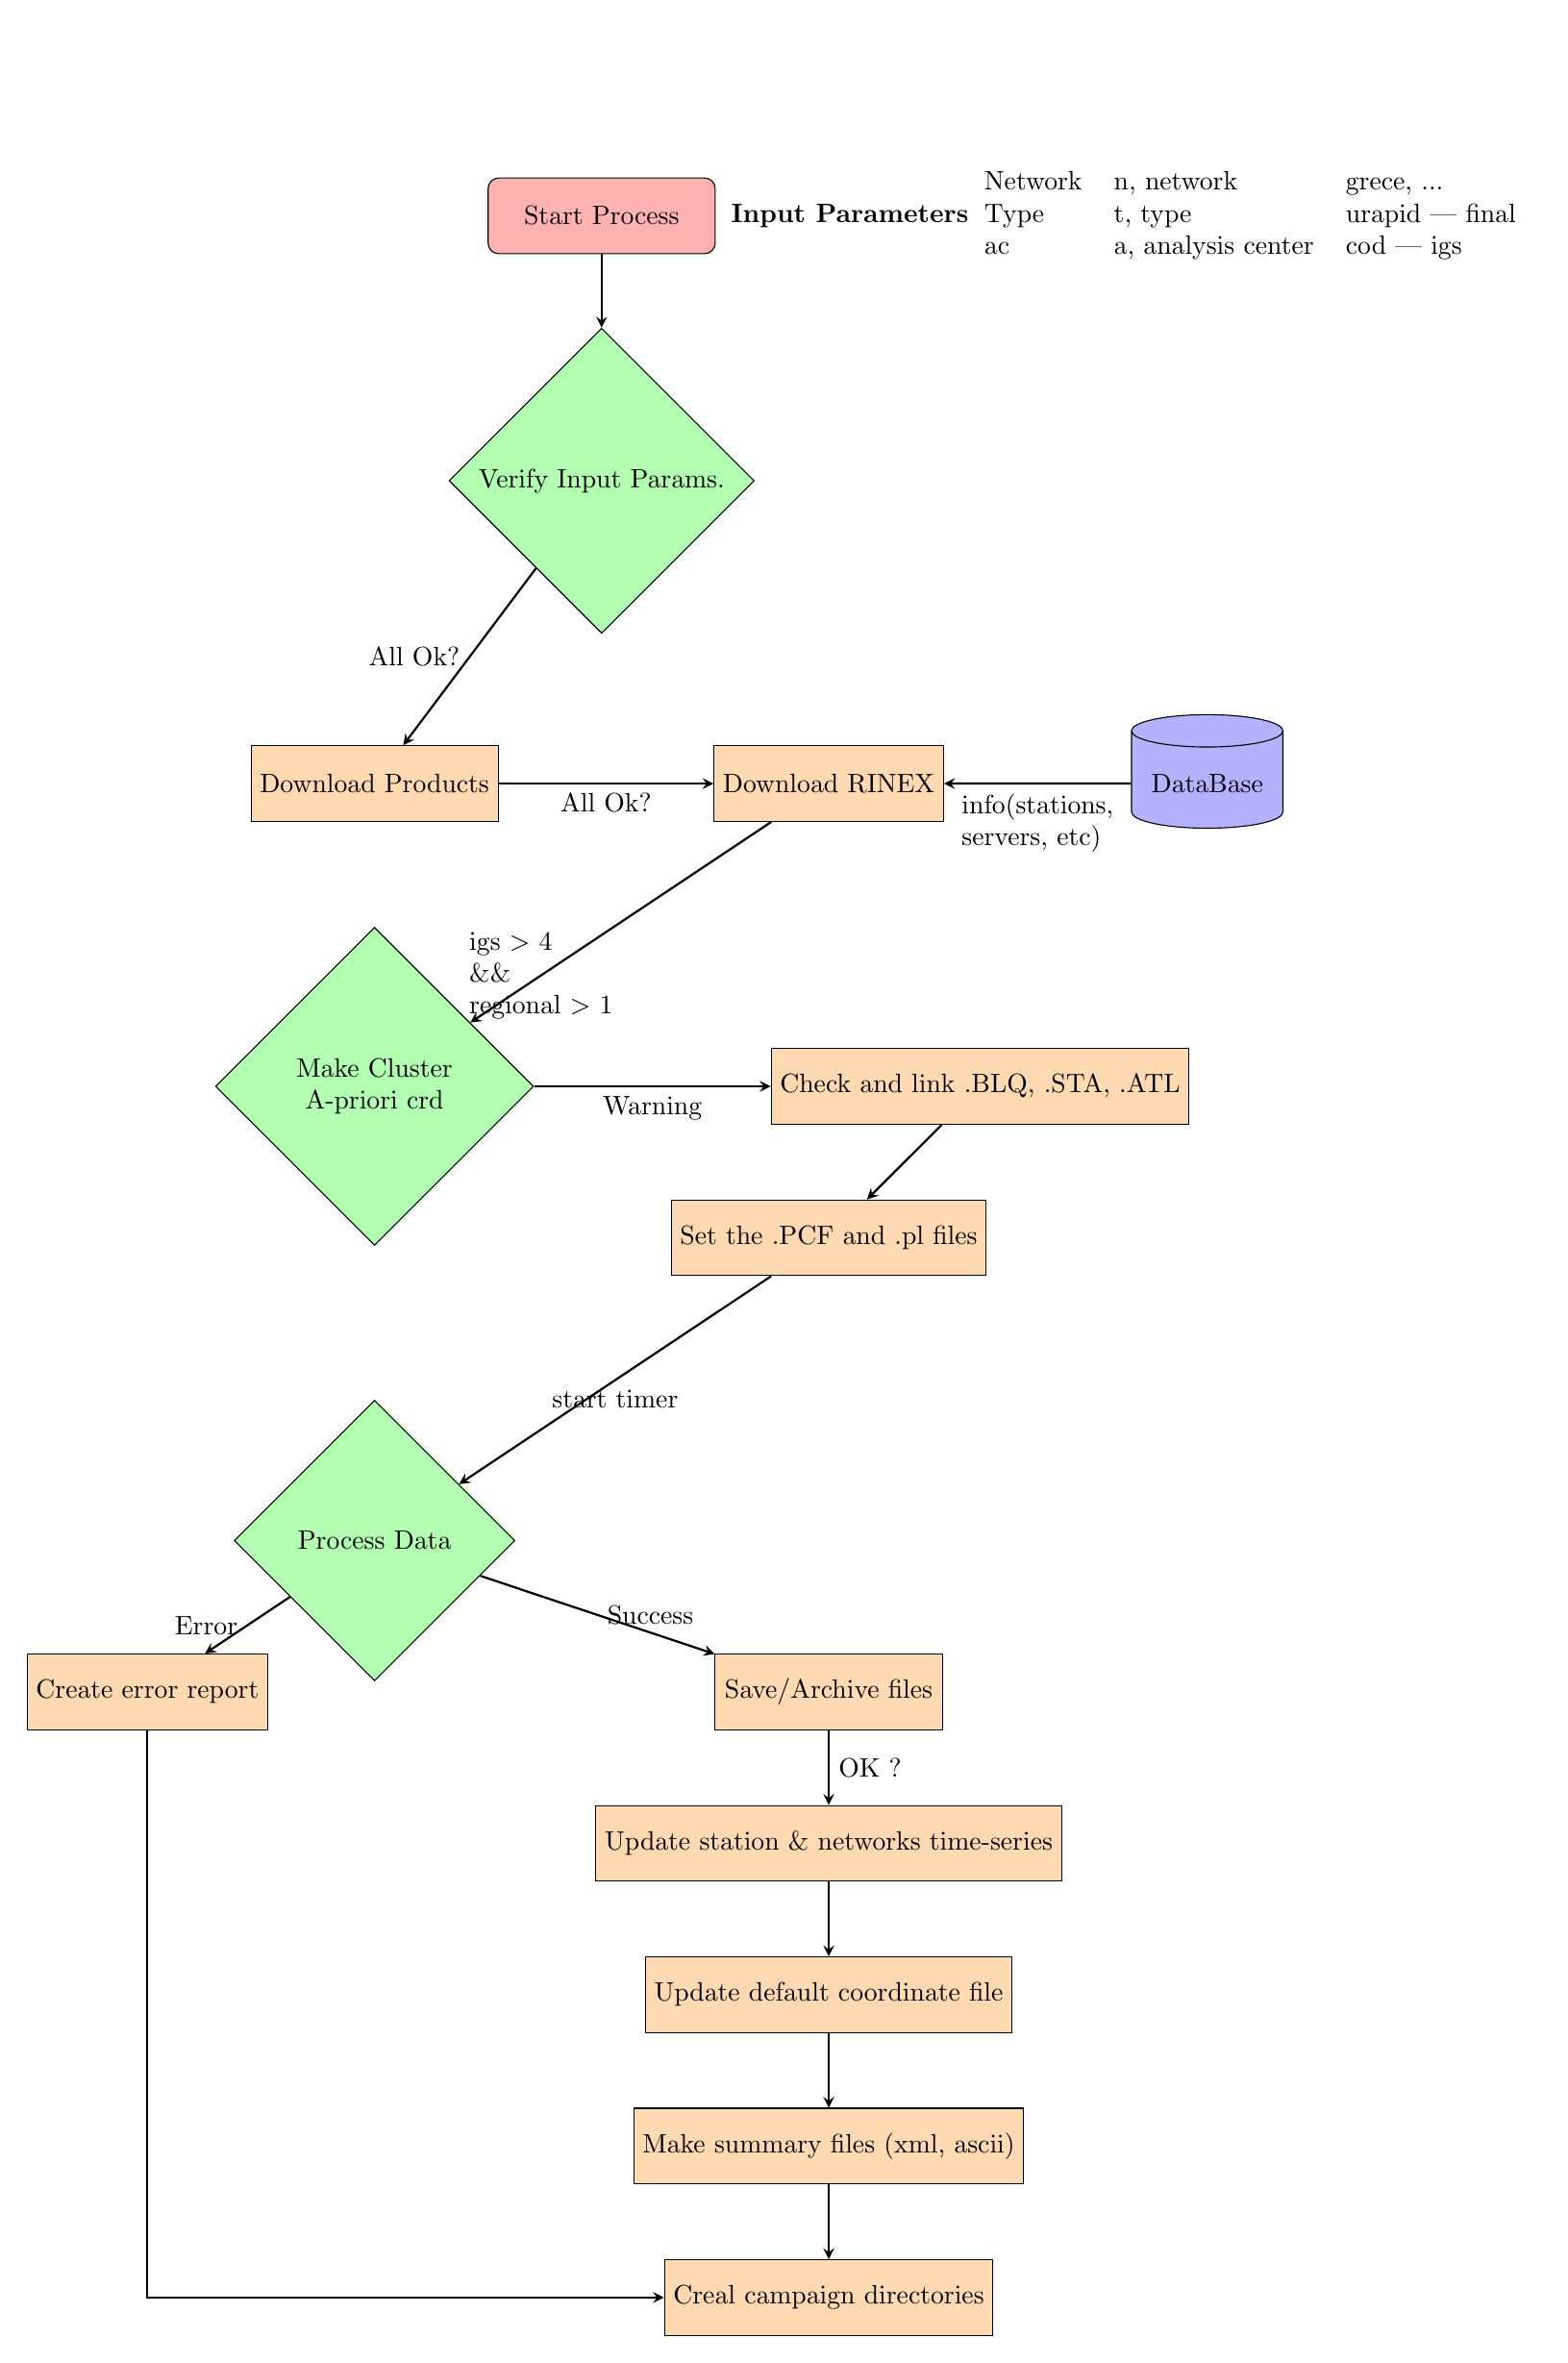
\begin{tikzpicture}[node distance=2cm]
%
% Define nodes
%
\node (start) [startstop] {Start Process};
\node (input_params) [textblock, right of=start, xshift=5cm] 
{\textbf{Input Parameters}\\
\begin{tabular}{l l l}
Network & n, network & grece, ...\\
Type    & t, type    & urapid | final\\
ac      & a, analysis center & cod | igs\\
\end{tabular}};
\node (verify)  [decision, below of=start, yshift=-1.5cm] {Verify Input Params.};
\node (dwnl_prd)  [process, below of=verify, xshift=-3cm, yshift=-2cm] {Download Products};
\node (dwnl_rnx)  [process, below of=verify, xshift=3cm, yshift=-2cm] {Download RINEX};
\node (datab) [database, below of=verify, xshift=8cm, yshift=-2cm] {DataBase};
\node (more)  [decision, below of=dwnl_rnx, xshift=-6cm, yshift=-2cm, text width=3cm] {Make Cluster\\A-priori crd};
\node (check) [process, right of=more, xshift=6cm] {Check and link .BLQ, .STA, .ATL};
\node (options) [process, below of=more, xshift=6cm] {Set the .PCF and .pl files};
\node (bpe)  [decision, below of=options, xshift=-6cm, yshift=-2cm, text width=3cm] {Process Data};
\node (erreport) [process, below of=bpe, xshift=-3cm] {Create error report};
\node (save) [process, below of=bpe, xshift=6cm] {Save/Archive files};
\node (upd-ts) [process, below of=save] {Update station \& networks time-series};
\node (upd-crd) [process, below of=upd-ts] {Update default coordinate file};
\node (summary) [process, below of=upd-crd] {Make summary files (xml, ascii)};
\node (clean) [process, below of=summary] {Creal campaign directories};
%
% Connect nodes
%
\draw [arrow] (start) -- (verify);
\draw [arrow] (verify) -- node[anchor=east] {All Ok?} (dwnl_prd);
\draw [arrow] (dwnl_prd) -- node[anchor=north] {All Ok?} (dwnl_rnx);
\draw [arrow] (datab) -- node[anchor=north,text width=2cm] {info(stations, servers, etc)} (dwnl_rnx);
\draw [arrow] (dwnl_rnx) -- node[anchor=north,text width=4cm] {igs $>$ 4\\ \&\& \\regional $>$ 1} (more);
\draw [arrow] (more) -- node[anchor=north] {Warning} (check);
\draw [arrow] (check) -- (options);
\draw [arrow] (options) -- node[anchor=north] {start timer}(bpe);
\draw [arrow] (bpe) -- node[anchor=east] {Error}(erreport);
\draw [arrow] (erreport) |- (clean);
\draw [arrow] (bpe) -- node[anchor=west] {Success}(save);
\draw [arrow] (save) -- node[anchor=west] {OK ?}(upd-ts);
\draw [arrow] (upd-ts) -- (upd-crd);
\draw [arrow] (upd-crd) -- (summary);
\draw [arrow] (summary) -- (clean);
\end{tikzpicture}
}

\section{Programs}
\subsection{ddprocess}
\label{ddprocess}

\subsubsection{Purpose}
\texttt{ddprocess.sh} is a bash (Shell) script to process a network in network mode, using the double-difference approach.\\
\textbf{Location:} \texttt{src/bash/ddprocess.sh}

\subsubsection{Usage}
\texttt{ddprocess -y YYYY -d DDD [OPTIONS]}\\

Switches:
\begin{itemize}
\item \texttt{-a --analysis-center=}[option]\\
Specify the analysis center. This can be either
\begin{enumerate}
\item igs, or
\item cod
\end{enumerate}
\underline{Default value: cod}.
\item \texttt{-b --bernese-loadvar=} /foo/bar/LOADGPS.setvar\\
Specify the Bernese LOADGPS.setvar file; this is needed to resolve the Bernese-related variables.
\item \texttt{-c --campaign=}[option]\\
Specify the campaign name. This name should be exactly the name of the campaign used within
Bernese. Inside the script it is truncated to upper-case, so the options
\texttt{--campaign=greece} and \texttt{--campaign=GREECE} are equivelant. For a list of all the files
depending on this variable, see \autoref{sec:ddprocess_notes}, Note 1.
Only specify the name of the campaign do \textbf{NOT} include the path.
\item \texttt{-d --doy=}[option]\\
Specify the day of year (as integer).
\item \texttt{-e --elevation-angle=}\\
Specify the elevation cut-off angle. The angle is expressed as integer in degrees.
\underline{Default value: 3}.
\item \texttt{-f --ion-products=}[option]\\
Specify (a-priori) ionospheric correction file identifier. If more than one, use a comma-seperated list 
(e.g. \texttt{-f FFG,RFG}). See \autoref{sec:ddprocess_notes}, Note 2.
\item \texttt{-i --solution-id=}[option]\\
Specify solution id (e.g. \texttt{FFG}). See \autoref{sec:ddprocess_notes}, Note 3.
\item \texttt{-l --stations-per-cluster=}[option]\\
Specify the number of stations per cluster. Input should be apositive integer.
\underline{Default value is 5}.
\item \texttt{-m --calibration-model=}[option]\\
The extension (model) used for antenna calibration files. This can be e.g. \texttt{I01, I05 or I08}. 
What you enter here, will be appended to the pcv filename (provided via the \texttt{-p} switch) and all 
calibration-dependent Bernese processing files (e.g. \texttt{SATELLITE.XXX}). 
See \autoref{sec:ddprocess_notes}, Note 4.
\item \texttt{-p --pcv-file=}[option]\\
Specify the PCV file to be used. Do not provide the extension (this is
automatically appended using the \texttt{-m} switch). See \autoref{sec:ddprocess_notes}, Note 4.
\item \texttt{-r --save-dir=}[option]\\
Specify directory where the solution will be saved; note that if the directory does not exist, 
it will be created.
\item \texttt{-s --satellite-system=}[option]\\
Specify the satellite system; this can be:
\begin{enumerate}
\item gps, or
\item mixed (i.e. gps+glonass)
\end{enumerate}
\underline{Default value is gps}.
\item \texttt{-t --solution-type=}[option]\\
Specify the solution type; this can be:
\begin{enumerate}
\item final, or
\item urapid
\end{enumerate}
\item \texttt{-u --update=}[option]\\
Specify which records/files should be updated; valid values are:
\begin{enumerate}
\item \texttt{crd} : update the default network crd file.
\item \texttt{sta} : update station-specific files, i.e. time-series records for the stations.
\item \texttt{ntw} : update update network-specific records.
\item \texttt{all} : all both the above.
\end{enumerate}
More than one options can be provided, in a comma seperated string e.g.
\texttt{--update=crd,sta}.
\item \texttt{-y --year=}[option]\\
Specify the year as a 4-digit integer.
\item \texttt{-x --xml-output}\\
Produce an xml (actually docbook) output summary report.
\item \texttt{--force-remove-previous}\\
Remove any files from the specified save directory (\texttt{-r --save-dir=}) prior to start 
of processing.
\item \texttt{--add-suffix=}[option]\\
Add a suffix (e.g. \texttt{\_GPS}) to saved products of the processing.
\item \texttt{-h --help}\\
Display (this) help message and exit.
\item \texttt{-v --version}\\
Dsiplay version and exit.
\end{itemize}


\subsubsection{Prerequisites}


\subsubsection{Exit Status}
On sucess, the program returns \texttt{0}.

\subsubsection{ToDo}
%\begin{tabular}{l l l}
%Date & What & Status\\
%\hline \\
%\end{tabular}

\subsubsection{Bugs}
Send reports to:\\
Xanthos Papanikolaou \href{mailto:xanthos@mail.ntua.gr}{mailto:xanthos@mail.ntua.gr}\\
Demitris Anastasiou  \href{mailto:danast@mail.ntua.gr}{mailto:danast@mail.ntua.gr}\\
Vangelis Zacharis  \href{mailto:vanzach@survey.ntua.gr}{mailto:vanzach@survey.ntua.gr}\\
\bigskip

%\begin{tabular}{l l l}
%Date & What & Status\\
%\hline \\
%\end{tabular}

\subsubsection{Notes}\label{sec:ddprocess_notes}
\begin{enumerate}[label=\arabic*]
\item A list of files are expected to be present in the tables directory, specified by
the campaign name. See \autoref{tab:ddprocess_notes}:

\begin{tabular}{l | l}\label{tab:ddprocess_notes}
Expected File & Linked to\\
\hline
 \$\{TABLES\}/pcv/\$\{PCV\_FILE\}       & \$\{X\}/GEN/\$\{PCV\_FILE\} \\
 \$\{TABLES\}/sta/\$\{CAMPAIGN\}.STA    & \$\{P\}/STA/\$\{CAMPAIGN\}.STA\\
 \$\{TABLES\}/blq/\$\{CAMPAIGN\}.BLQ    & \$\{P\}/STA/\$\{CAMPAIGN\}.BLQ\\
 \$\{TABLES\}/atl/\$\{CAMPAIGN\}.ATL    & \$\{P\}/STA/\$\{CAMPAIGN\}.ATL\\
 \$\{TABLES\}/crd/\$\{CAMPAIGN\}.igs    & \\
 \$\{TABLES\}/crd/\$\{CAMPAIGN\}.epn    & \\
 \$\{TABLES\}/crd/\$\{CAMPAIGN\}.reg    & \\
\hline
\end{tabular}
\item The ionospheric correction file, must be in the Bernese-specific ION format.
These files should reside in the product area, specified by the variable \$\{PRODUCT\_AREA\}
stored as \$\{PRODUCT\_AREA\}/YYYY/DDD/XXXYYDDD0.ION.Z, where \texttt{XXX} is the solution identifier
specified by the \texttt{-f} option.\\
If none of these files are found (or if the \texttt{-f} switch is not used), then the script
will try to download a Bernese-specific ION file from CODE's ftp, using the program
wgetion. This downloaded files can be final, rapid or ultra-rapid.
\item The solution id will have an effect on the naming of the Final, Preliminary
and Size-Reduced solution files. If e.g. the solution-id is set to \texttt{NTA}, then
the Final solution files will be named \texttt{NTA}, the preliminary \texttt{NTP} 
and the size-reduced \texttt{NTR}.
\item The pcv file must reside in the \texttt{tables/pcv} folder, and will be linked by the
script to the \{\%GEN\} directory. Do not provide the extension; it will be automatically
generated using the pcv file and the extension given via the calibration model (\texttt{-m}).
E.g. using \texttt{-p GRE\_PCV} and \texttt{-m I08}, then the script will search for the pcv file
\$\{TABLES\}/pcv/GRE\_PCV.I08.
\end{enumerate}
\subsection{rnxdwnl}
\label{rnxdwnl}

\subsubsection{Purpose}
\texttt{rnxdwnl.py} is a Python script to download RINEX files.\\
\textbf{Location:} \texttt{src/python/rnxdwnl.py}

\subsubsection{Usage}
\texttt{rnxdwnl -y YYYY -d DDD [OPTIONS]}\\

Switches:
\begin{itemize}
\item \texttt{-s, --stations=} station1,stations2,...\\
Specify a comma-seperated list of stations to be downloaded. The stations specified here, 
must be included in the database. The name of stations specified, must be the one
used by DSO (a 4-char string). In some, rare cases, this may not match the 'official'
4-char name of the station. When the rinex file is searched for on the web, the
'official' name will be used.
\item \texttt{-n, --networks=} network1,network2,...\\
Specify a comma-seperated list of networks. Every station, belonging to these
networks will (try to) be downloaded. The name of the network(s) specified, must 
match valid networks in the database.
\item \texttt{-y, --year=} YYYY\\
Specify the year for which the RINEX are requested. This must be a (valid),
4-digit integer.
\item \texttt{-d, --doy=} DDD\\
Specify the day of year for which the RINEX are requested. This must be a (valid), integer.
\item \texttt{-f, --force-remove}\\
By default, if the RINEX to be downloaded already exists, with size $>$ 0, then
the downloading step is not performed (other steps -if specified- are perfored normaly).
If this switch is turned on, then if a file exists,
named exactly as the one to be downloaded, then this file is removed and a normal,
download is performed.
\item \texttt{-u, --uppercase}\\
If turned on, the downloaded RINEX file(s) will be truncated to upper-case.
\item \texttt{-p, --path=} /foo/bar\\
Specify the directory (path) where the downloaded files will be downloaded to.
\item \texttt{-z, --uncompress}\\
Uncompress the downloaded RINEX file(s). Note that this will only work for UNIX compressed '.Z' files.
\end{itemize}

\subsubsection{Prerequisites}
The Python library MySQLdb must be installed and available for importing.\\

The program needs to connect to a (MySQL) database called \index{procsta}\texttt{procsta}, 
and make various queries
about the stations, networks, servers, etc. The structure of this database
is strict, cause the queries are hardcoded in the source code of this program.\\

For more information on the used database, ask \href{mailto:danast@mail.ntua.gr}{Mitsos}.\\

The program is designed to work on UNIX-like systems. It will call the Shell to issue commands (like
downloading, compressing, etc). Depending on the specific use, the following may be required:
\begin{itemize}
\item \texttt{compress} and/or \texttt{uncompress} utilities; needed to compress or uncompress
UNIX-compressed files (i.e. \texttt{.Z}).
\item \texttt{wget} needed to download remote files, when the protocol is \texttt{http}, \texttt{ftp}, or \texttt{https}.
\item \texttt{scp} needed to download remote files, when the protocol is \texttt{ssh}. Note that if a non-standard port
is used for \texttt{ssh}, then it must be hardcoded into the source code. Also, the remote and server sites, must be able to
connect without using explicit passwords (they must hold the ssh keys).
\end{itemize}

\subsubsection{Exit Status}
On sucess, the program returns \texttt{0}.

\subsubsection{ToDo}
\begin{tabular}{l l l}
Date & What & Status\\
\hline \\
11,Jun,15  & add switch for excluding certain stations & Waiting ...\\
\end{tabular}

\subsubsection{Bugs}
Send reports to:\\
Xanthos Papanikolaou \href{mailto:xanthos@mail.ntua.gr}{mailto:xanthos@mail.ntua.gr}\\
Demitris Anastasiou  \href{mailto:danast@mail.ntua.gr}{mailto:danast@mail.ntua.gr}\\
Vangelis Zacharis  \href{mailto:vanzach@survey.ntua.gr}{mailto:vanzach@survey.ntua.gr}\\
\bigskip

\begin{tabular}{l l l}
Date & What & Status\\
\hline \\
11,Jun,15  & Add help switch & Waiting ...\\
\end{tabular}
\subsection{syncwbern52}
\label{syncwbern52}

\subsubsection{Purpose}
\texttt{syncwbern52.py} is a bash (Shell) script to synchronize (mirror) a local Bernese \texttt{GEN}
directory, with the remote one, which can be found at AIUB's ftp server
\url{fpt://ftp.unibe.ch/aiub/BSWUSER52/GEN/}.\\
\textbf{Location:} \texttt{src/bash/syncwbern52.sh}

\subsubsection{Usage}
\texttt{syncwbern52 [OPTIONS]}\\
at least either \texttt{--target-directory=} or \texttt{--bernese-loadvar=}
must be specified as command line arguments.


Switches:
\begin{itemize}
\item \texttt{-t --target-directory=} /foo/bar\\
Specify the (local) target directory in localhost (See \autoref{sec:syncwbern52_notes}, Note 1).
\item \texttt{-b --bernese-loadvar=} /foo/bar/LOADGPS.setvar\\
Specify a Bernese source file (i.e. the file \texttt{BERN52/GPS/EXE/LOADGPS.setvar}) 
which can be sourced; if such a file is set, then the local target 
directory is defined by the variable \$X/GEN. (See \autoref{sec:syncwbern52_notes}, Note 1)
\item \texttt{-o --logfile=} [logfile]\\
Specify log file. \underline{Default value is /dev/null}.
\item \texttt{-q --quite}\\
Do not show progress on screen.
\item \texttt{-s --stamp-file=} [stampfile]\\
Specify a file where the time stamp of current run will be written, 
so that the user can keep track of when the last mirroring was done.
\item \texttt{-h --help}\\
Display (this) help message and exit.
\item \texttt{-v --version}\\
Dsiplay version and exit.
\end{itemize}

\subsubsection{Prerequisites}
\begin{itemize}
\item \texttt{getopt},
\item \texttt{lftp}, 
\item \texttt{hash}
\end{itemize}

\subsubsection{Exit Status}
On sucess, the program returns \texttt{0}.\\
Else, the return status is $>$0.

\subsubsection{ToDo}
%\begin{tabular}{l l l}
%Date & What & Status\\
%\hline \\
%\end{tabular}

\subsubsection{Bugs}
Send reports to:\\
Xanthos Papanikolaou \href{mailto:xanthos@mail.ntua.gr}{mailto:xanthos@mail.ntua.gr}\\
Demitris Anastasiou  \href{mailto:danast@mail.ntua.gr}{mailto:danast@mail.ntua.gr}\\
Vangelis Zacharis  \href{mailto:vanzach@survey.ntua.gr}{mailto:vanzach@survey.ntua.gr}\\
\bigskip

%\begin{tabular}{l l l}
%Date & What & Status\\
%\hline \\
%\end{tabular}

\subsubsection{Notes}\label{sec:syncwbern52_notes}
\begin{enumerate}[label=\arabic*]
\item Note that if both \texttt{-t} and \texttt{-b} switches are used, 
the target directory is the one specified by the \texttt{-b} option 
(i.e. using the LOADGPS.setvar file).\\
\item All files with \texttt{.EPH} extension will be excluded from synchronization.
\end{enumerate}
\subsection{updatecrd}
\label{updatecrd}

\subsubsection{Purpose}
\texttt{updatecrd.py} is a Python script used to update the (cartesian) coordinates in a
Bernese-formated \texttt{.CRD} file, using a second \texttt{.CRD} file as reference.\\
\textbf{Location:} \texttt{src/python/updatecrd.py}

\subsubsection{Usage}
\texttt{updatecrd -r [.CRD-file] -u [.CRD-file] [OPTIONS]}\\
at least \texttt{--update-file=} and \texttt{--reference-file=}
must be specified as command line arguments.\\

Switches:
\begin{itemize}
\item \texttt{-u --update-file=} [.CRD-file]\\
The \texttt{.CRD} file to be updated.
\item \texttt{-r --reference-file=} [.CRD-file]\\
The \texttt{.CRD} file to be used as reference.
\item \texttt{-s --stations=} [station1,station2]\\
A comma-seperated list of stations, whose coordinates should be updated. 
If not specified, then all stations found in the file-to-be-updated will be
updated, if they are macthed in the reference .CRD file.
\item \texttt{-f --flags=} [A,W]\\
Only update stations flaged with specific characters in the 
reference file. The flags should be specified using a comma-seperated list, 
e.g. \texttt{--flags=W,A}. If this switch is not specified, 
all matching stations will be updated regardless of their flags.
\item \texttt{--include-unmatched}\\
The final output CRD file, will contain all the stations recorded
in the reference file (either matched or not).
\item \texttt{--delete-unmatched}\\
By default, all stations recorded in the file-to-be-updated will be included
in the resulting file. If this (\texttt{--delete-unmatched}) switched is turned on,
then stations that are not matched in the reference file will not be included in the
resulting file.
\item \texttt{--no-marker-number}\\
If specified, the marker number will not be used when trying to match
stations (i.e. \texttt{YEBE 13420M001} will be matched to \texttt{YEBE}).
\item \texttt{-h --help}\\
Display (this) help message and exit.
\item \texttt{-v --version}\\
Dsiplay version and exit.
\end{itemize}

\subsubsection{Prerequisites}
\begin{itemize}
\item \texttt{bernutils.berncrd} Python (library) module.
\end{itemize}

\subsubsection{Exit Status}
On sucess, the program returns \texttt{0}.\\
Else, the return status is $>$0.

\subsubsection{ToDo}
%\begin{tabular}{l l l}
%Date & What & Status\\
%\hline \\
%\end{tabular}

\subsubsection{Bugs}
%Send reports to:\\
%Xanthos Papanikolaou \href{mailto:xanthos@mail.ntua.gr}{mailto:xanthos@mail.ntua.gr}\\
%Demitris Anastasiou  \href{mailto:danast@mail.ntua.gr}{mailto:danast@mail.ntua.gr}\\
%Vangelis Zacharis  \href{mailto:vanzach@survey.ntua.gr}{mailto:vanzach@survey.ntua.gr}\\
See \autoref{subsec:bugs1}.
\bigskip

\begin{tabular}{l l l}
Date & What & Status\\
\hline \\
JUN, 2015 & help and version switch not working. Fix & Waiting ...\\
\end{tabular}
\subsection{getvmf1}
\label{getvmf1}

\subsubsection{Purpose}
\texttt{getvmf1.py} is a Python script to download VMF1 (i.e. Vienna Mapping Function 1)
grid files. These files are located on the web at \url{http://ggosatm.hg.tuwien.ac.at}.
Grid files older than today are always placed in 
\url{http://ggosatm.hg.tuwien.ac.at/DELAY/GRID/VMFG/YYYY} while prediction files (including
today and forward) are placed in \url{http://ggosatm.hg.tuwien.ac.at/DELAY/GRID/VMFG_FC/YYYY}.

The grid files hold values per 6 hours (so we have 4 files per day), at 00, 06, 12 and 18
hours and they are named as \texttt{VMFG\_YYYYMMDD.HSS}, where:
\begin{itemize}
    \item \texttt{YYYY} is the year,
    \item \texttt{MM} is the month,
    \item \texttt{DD} is the day of month and
    \item \texttt{SS} is the hour (00, 06, 12 or 18)
\end{itemize}

Note that the grid files previous than 01/01/2009 are compressed in \texttt{.gz} format;
the routine will automatically uncompress these files.

\subsubsection{Usage}
\texttt{getvmf1 -y [year] -d [doy] [OPTIONS]}\\
at least \texttt{--year=} and \texttt{--doy=}
must be specified as command line arguments.\\

Switches:
\begin{itemize}
\item \texttt{-y --year=}[YYYY]\\
The \texttt{YEAR} for which the grid file is needed.
\item \texttt{-d --doy=}[Day Of Year]\\
The \texttt{day of year} for which the grid file is needed.
\item \texttt{-r --hour=}[Hour]\\
If we only want a single grid file to cover a certain time interval, then this switch
can be used. The \texttt{hour} argument should be a valid integer of float in the range
[0,24).
\item \texttt{-o --outdir=}[output directory]\\
Specify the directory where the downloaded file(s) will be saved.
\item \texttt{-h --help}\\
Display (this) help message and exit.
\item \texttt{-v --version}\\
Dsiplay version and exit.
\end{itemize}

\subsubsection{Prerequisites}
\begin{itemize}
\item \texttt{bernutils.berncrd} Python (library) module.
\end{itemize}

\subsubsection{Exit Status}
On sucess, the program returns \texttt{0}.\\
Else, the return status is $>$0.\\


The routine will also report the list of downloaded and saved files to \texttt{stdout}, e.g.
\begin{Verbatim}[fontsize=\scriptsize]
$> getvmf1 -y 2007 -d 10 -o /foo/bar/data
Downloaded http://ggosatm.hg.tuwien.ac.at/DELAY/GRID/VMFG/2007/VMFG_20070110.H00.gz to /foo/bar/data/VMFG_20070110.H00
Downloaded http://ggosatm.hg.tuwien.ac.at/DELAY/GRID/VMFG/2007/VMFG_20070110.H06.gz to /foo/bar/data/VMFG_20070110.H06
Downloaded http://ggosatm.hg.tuwien.ac.at/DELAY/GRID/VMFG/2007/VMFG_20070110.H12.gz to /foo/bar/data/VMFG_20070110.H12
Downloaded http://ggosatm.hg.tuwien.ac.at/DELAY/GRID/VMFG/2007/VMFG_20070110.H18.gz to /foo/bar/data/VMFG_20070110.H18
\end{Verbatim}

\subsubsection{ToDo}
\begin{tabular}{l l l}
Date & What & Status\\
\hline \\
20,Jul,15  & add switch for help and version & Waiting ...\\
\end{tabular}

\subsubsection{Bugs}
Send reports to:\\
Xanthos Papanikolaou \href{mailto:xanthos@mail.ntua.gr}{mailto:xanthos@mail.ntua.gr}\\
Demitris Anastasiou  \href{mailto:danast@mail.ntua.gr}{mailto:danast@mail.ntua.gr}\\
Vangelis Zacharis  \href{mailto:vanzach@survey.ntua.gr}{mailto:vanzach@survey.ntua.gr}\\
\bigskip

\begin{tabular}{l l l}
Date & What & Status\\
\hline \\
JUN, 2015 & help and version switch not working. Fix & Waiting ...\\
\end{tabular}

\clearpage
\addcontentsline{toc}{chapter}{Index}
\printindex

\end{document}
